\chapter{Introduction}
\section{Printing Special Characters in the text area}
\subsection{Printing special characters with escape-sequence}
 Special Characters \\ % Double backslash is used for newline 
  Percentage Symbol - 100\%  \\ % Only percentage sign is used for comment 
  Dollar Sign - \$5 \\
  Hash Sign - \#1024  \\
  Ampersand Sign - \&4001   \\
  Open brace bracket - \{  \\
  Close brace bracket - \}  \\
 

%\begin{figure}[H]
 % \centering
  %  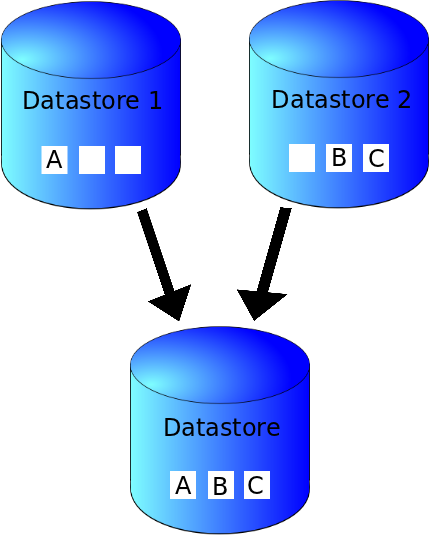
\includegraphics[height= 5cm, width=10cm]{project/images/data-sync}
 % \caption{\textbf{IMAGE CAPTION}}
%\end{figure}

\subsection{Special Characters with Key words}
 Special Characters \\ % Double backslash is used for newline 
  backslash  - something \textbackslash something \\
  bar        - ls -l\textbar less \\
  greater than -  10 \textgreater 5 \\
  less than -  5 \textless 10 \\
  dash 1 - inter\textendash val \\
  dash 2   -  \textemdash \\
  underscore -  \verb|Samp_Dist_Corr_| \\
  forward slash   - /
  
\subsection{Paragraph and removing extra spaces}

The end of a paragraph is specified by a blank line in the input.                                   In other words, whenever you want to start a new paragraph, just leave a blank line and proceed. 

\noindent We have seen that to typeset                                  something in \LaTeX, we type in                        the text to be typeset together with some \LaTeX\ commands.                                   Words must be separated by spaces (does not matter how many) and lines maybe broken arbitrarily. 

We can also use \par to break paragraph. 

\paragraph{Concluding Remarks:}
The end of a paragraph is specified by a \emph{blank line} in the input. In other words, whenever you want to start a new paragraph, just leave a blank line and proceed.

\subsection{Single Quotes and Double Quotes}

This is  'single quotes' and this is ``double quotes''. We can also use \lq quotes \rq for single quotes and \lq\lq double quotes\rq\rq .

\subsection{Special Symbols}

You can print LATEX as \LaTeX. \\
You can add additional vertical space \\ [2.0cm]
between two lines. \\

\noindent Greek Alphabets \\
alpha  -  $\alpha$ \\
beta   - $\beta$  \\
Beta   -   B  \\
gamma  -$\gamma$ \\
Gamma  - $\Gamma$ \\
Lambda - $\Lambda$ \\
omega  - $\omega$ \\
Theta  - $\Theta$ \\


\subsection{Text Positioning - Left Justify , Center , Right Justify }

\begin{center}
The \TeX nical Institute\\[.75cm]
Certificate
\end{center}
This is to certify that Mr. N. O. Vice has undergone a
course at this institute and is qualified to be a \TeX nician.
\begin{flushright}
The Director\\
The \TeX nical Institute
\end{flushright}


\subsection{ }


  